\chapter{Construção da ontologia}

  \section{Metodologia utilizada para construção}
    
    APRESENTAR AQUI A METODOLOGIA ESCOLHIDA PARA A CONSTRUÇÃO DA ONTOLOGIA (Ontology 101).
    
  \section{Construção da ontologia}
    
    \subsection{Escopo da ontologia}
    
    \subsection{Ontologias encontradas}
   
        A fim de não ter retrabalho desnecessário, e de usar os conhecimentos previamente
  pesquisados por outros grupos de pesquisa, este grupo procurou em bases de periódicos e no
  próprio Google por ontologias que já existissem, e pudessem retratar de forma semântica os
  acidentes listados no software “Pé na Estrada”. As consultas muitas vezes não retornaram
  resultados satisfatórios, mas foi possível encontrar duas ontologias muito parecidas.
  
  De posse das ontologias, é possível observar a similaridade entre as duas encontradas,
  até por que as duas são empregadas em soluções tecnológicas parecidas. Sua aplicação
  consiste na organização das informações de acidentes em estradas, para que as informações de
  um acidente de trânsito sejam devidamente transmitidas em redes veiculares Ad hoc, ou
  VANETs \cite{barrachina12}. Essas redes usam os carros como nós de uma rede para
  trafegar informações, que podem ser analisados e registrados em banco de dados. Na
  aplicação dos projetos encontrados ela também tem a utilidade de alertar ambulâncias, ou
  hospitais próximos que possam prestar socorro de forma rápida e eficiente. As duas
  ontologias possuem as mesmas entidades e seus relacionamentos são idênticos, evidenciando
  a robustez das mesmas. A diferença está nos atributos das entidades, com a adição de diversos
  campos que fornecem informações valiosas para a correta identificação do acidente de
  trânsito \cite{villalba14}.
  
  Desta forma, as duas ontologias são tomadas como base para o contexto deste projeto,
  pois se adequam muito bem dentro dos objetivos almejados. Será proposta a adição de uma
  entidade, de forma que seja possível também captar informações sobre a rodovia a qual o
  acidente ocorreu, diferentemente da entidade ambiente (“environment”), que procura detalhar
  as condições no momento do acidente. A entidade rodovia terá atributos que irão guardar as
  informações daquela rodovia, relacionadas ao contexto do projeto. O detalhamento dessa
  entidade será conduzido no trabalho seguinte.
  
  As duas ontologias podem ser vistas na Figura \ref{fig:ontologia1} e na Figura \ref{fig:ontologia2}.
  
  \begin{figure}[!htb]
    \centering
    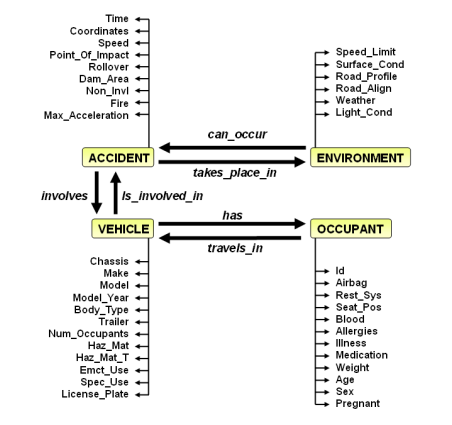
\includegraphics[scale = 0.5]{ontologia1}
    \caption[Componentes da ontologia]{Componentes da ontologia. Fonte: \cite{villalba14}}
    \label{fig:ontologia1}
  \end{figure}
  
    \begin{figure}[!htb]
    \centering
    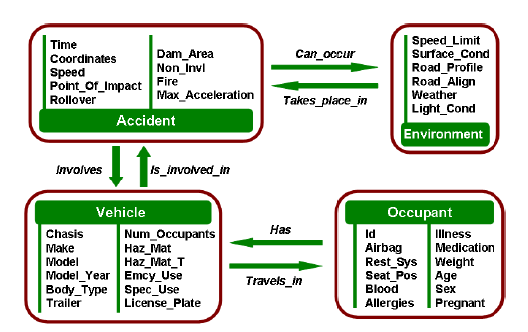
\includegraphics[scale = 0.5]{ontologia2}
    \caption[Componentes da ontologia CAOVA]{Componentes da ontologia CAOVA. Fonte: \cite{barrachina12}}
    \label{fig:ontologia2}
  \end{figure}
      
    \subsection{Estrutura da ontologia}
      
      \subsubsection{Classes}
	
	\emph{\textit{Card Sorting}}
	  Falar da técninca do Card Sorting aqui, que foi utilizada para a definição das classes (sei la)...
      
    \subsubsection{Propriedades}
	
	
    \subsubsection{Modelo conceitual da ontologia}
    
      
  Como não foi possível encontrar o código OWL das ontologias pesquisadas, a equipe decidiu aproveitar a
  modelagem conceitual feita nos trabalhos encontrados. A partir desses modelos, foi construído o modelo 
  para a ontologia, ilustrado na figura \ref{fig:modelo_conceitual_ontologia}.
  
  \begin{figure}[!htb]
    \centering
    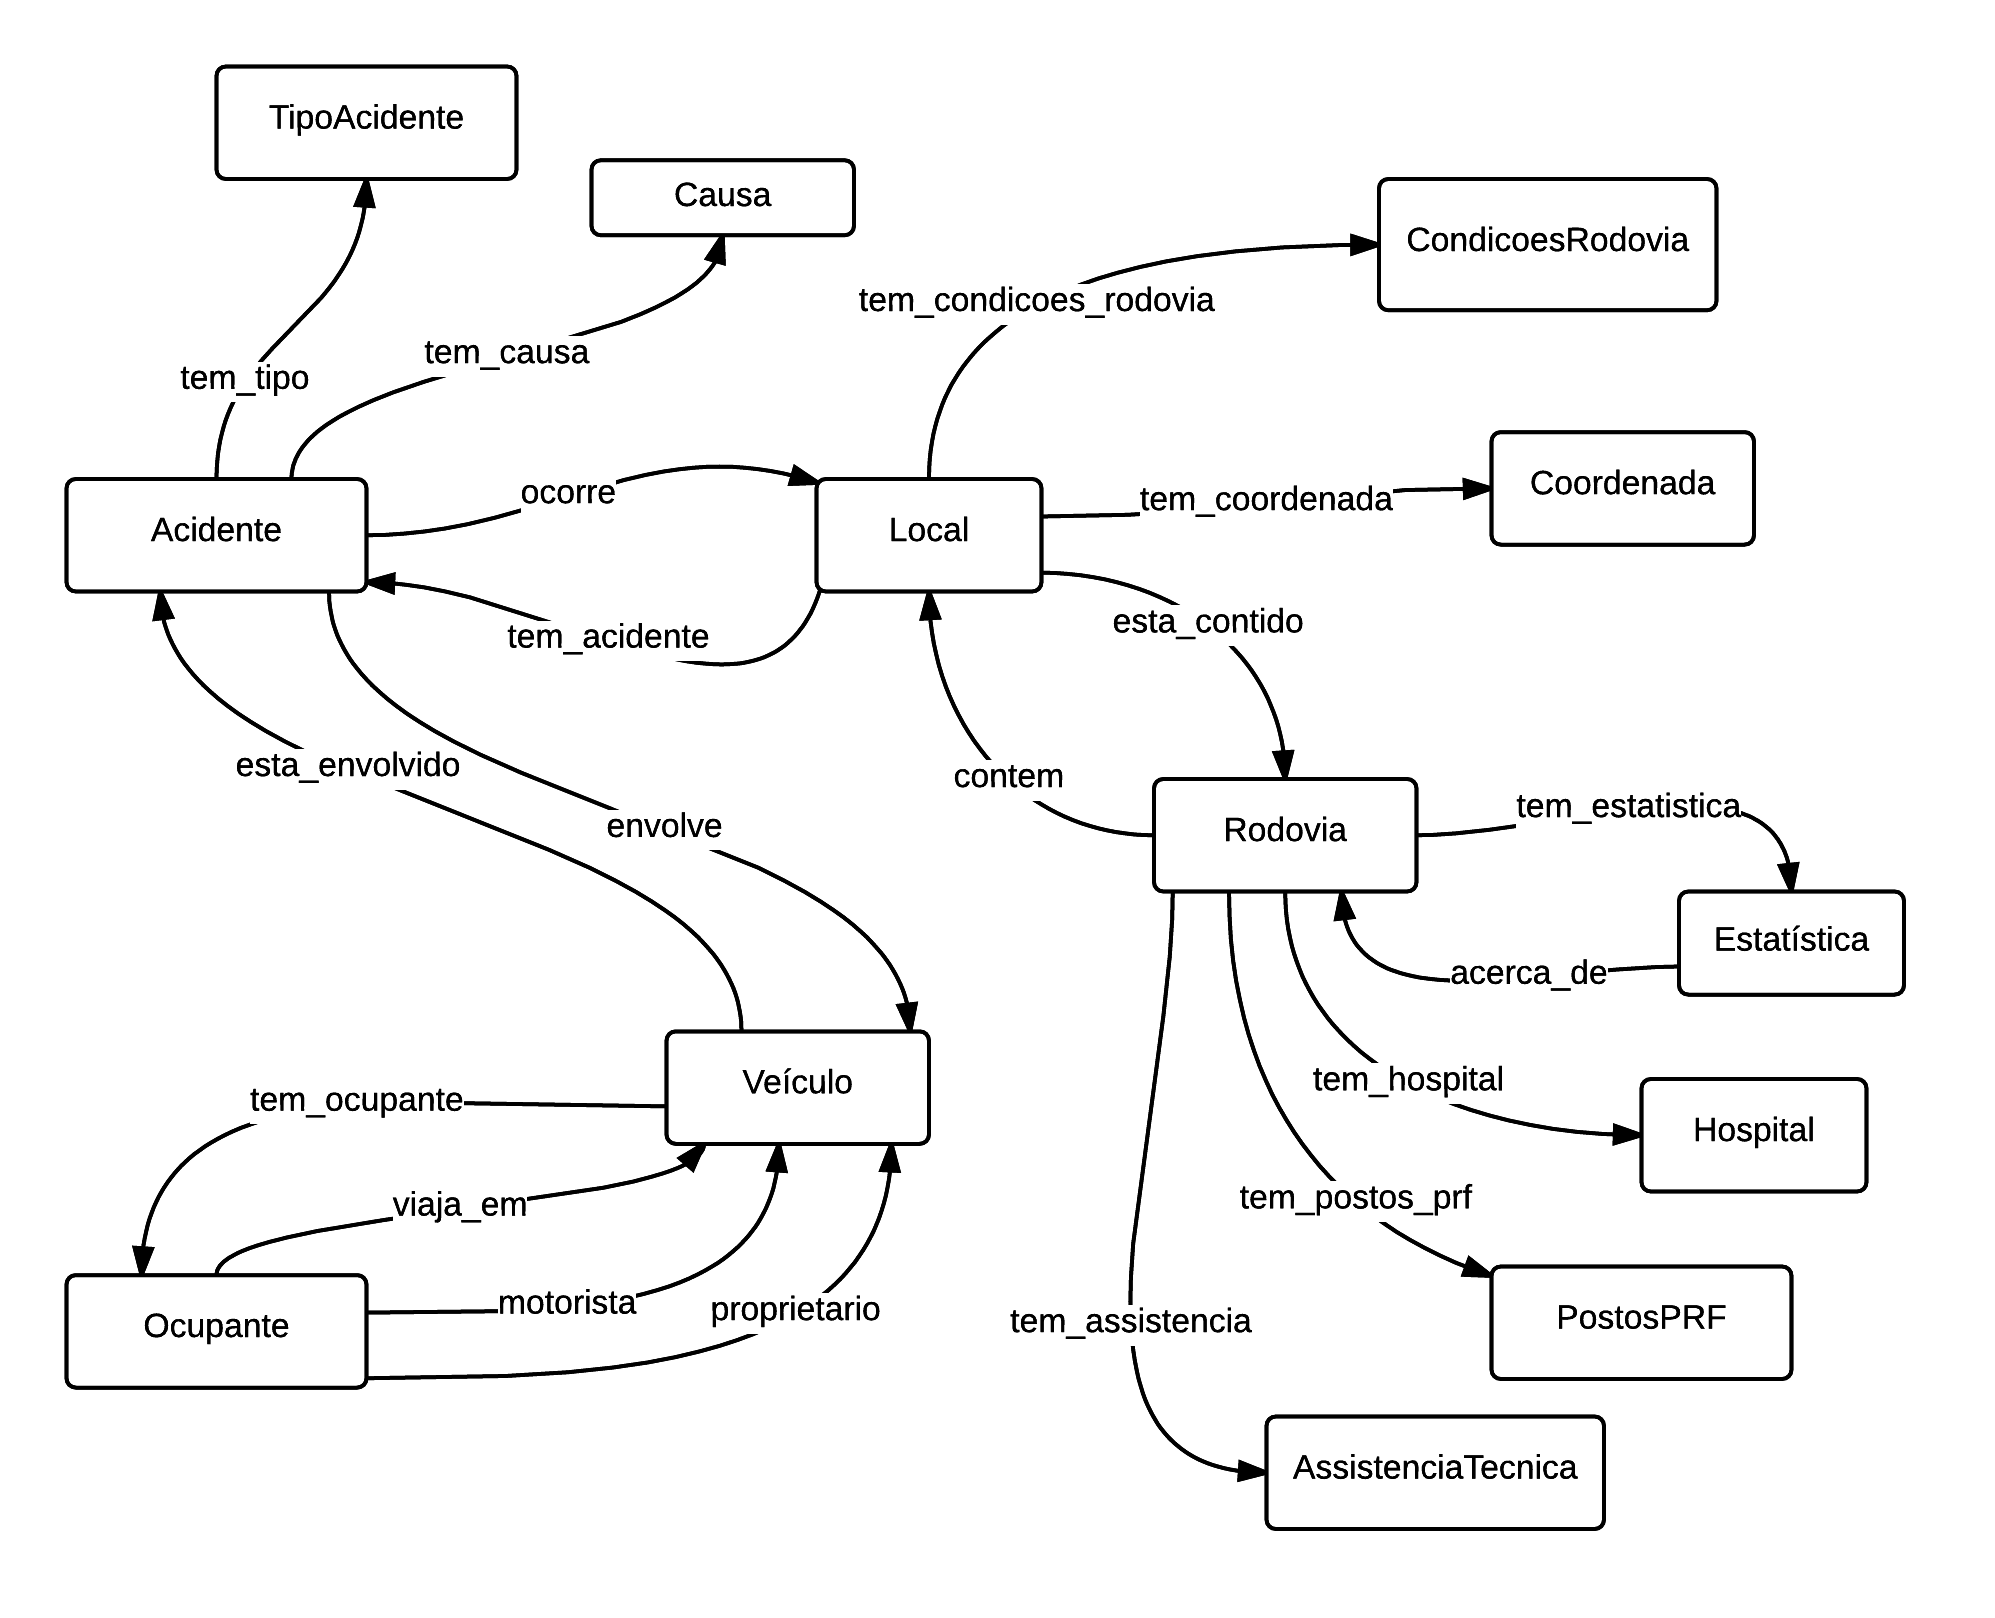
\includegraphics[scale = 0.23]{modelo_conceitual_ontologia}
    \caption[Modelo conceitual da ontologia]{Modelo conceitual da ontologia a ser construída}
    \label{fig:modelo_conceitual_ontologia}
  \end{figure}
    
      
  

  